\clearpage
%----------------------------------------------------------------------------
\appendix
%----------------------------------------------------------------------------
\chapter*{\fuggelek}\addcontentsline{toc}{chapter}{\fuggelek}
\setcounter{chapter}{\appendixnumber}
%\setcounter{equation}{0} % a fofejezet-szamlalo az angol ABC 6. betuje (F) lesz
\numberwithin{equation}{section}
\numberwithin{figure}{section}
\numberwithin{lstlisting}{section}
%\numberwithin{tabular}{section}


\section{Precision-recall curves and tracking performances}

\begin{figure}[h]
    \captionsetup{width=\textwidth}
    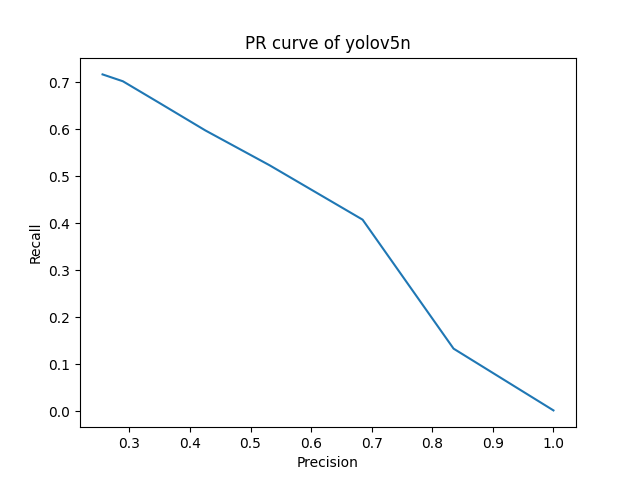
\includegraphics[width=0.49\textwidth]{figures/yolov5n.png}
    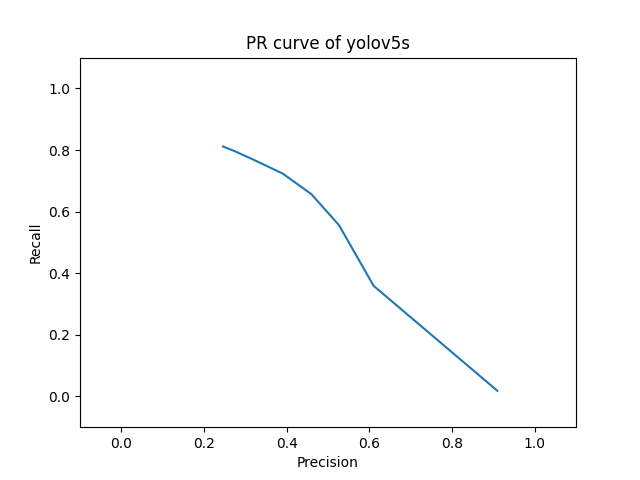
\includegraphics[width=0.49\textwidth]{figures/yolov5s.png} \\
    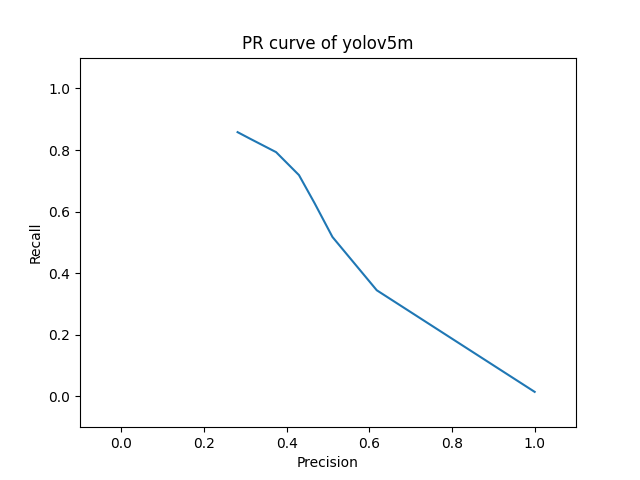
\includegraphics[width=0.49\textwidth]{figures/yolov5m.png}
    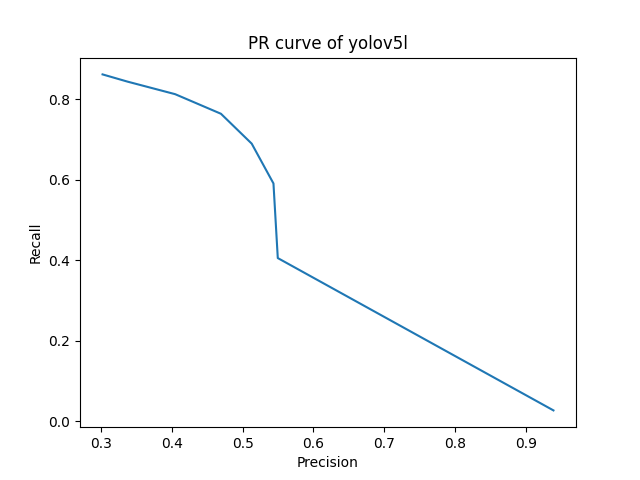
\includegraphics[width=0.49\textwidth]{figures/yolov5l.png} \\
    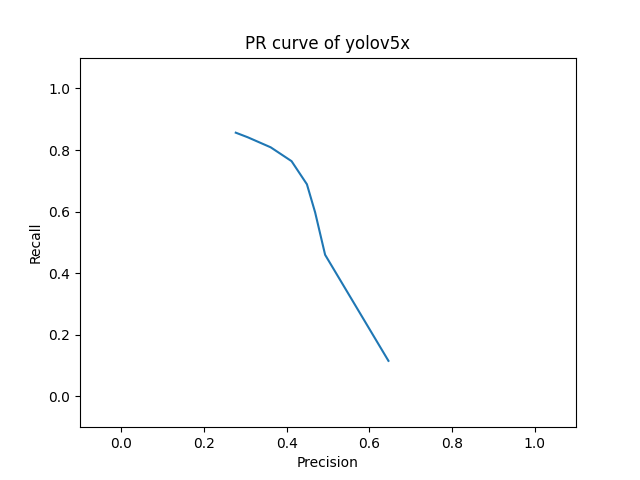
\includegraphics[width=0.49\textwidth]{figures/yolov5x.png}
    \caption{The PR curves of the five YOLO models.}
    \label{fig:pr_yolo}
\end{figure}

\clearpage

\begin{figure}[h]
    \captionsetup{width=\textwidth}
    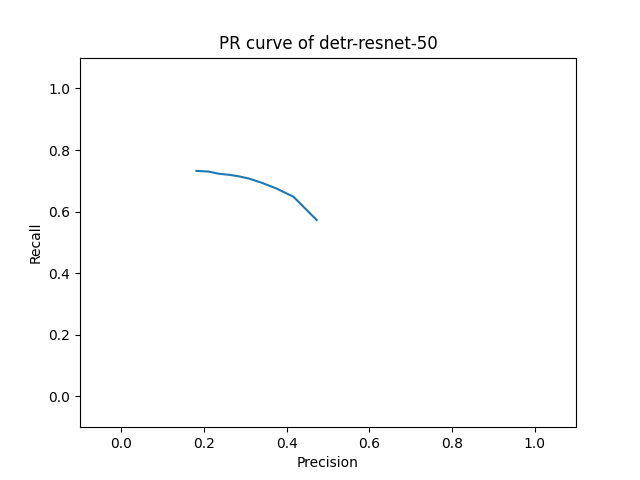
\includegraphics[width=0.49\textwidth]{figures/detr-resnet-50.png}
    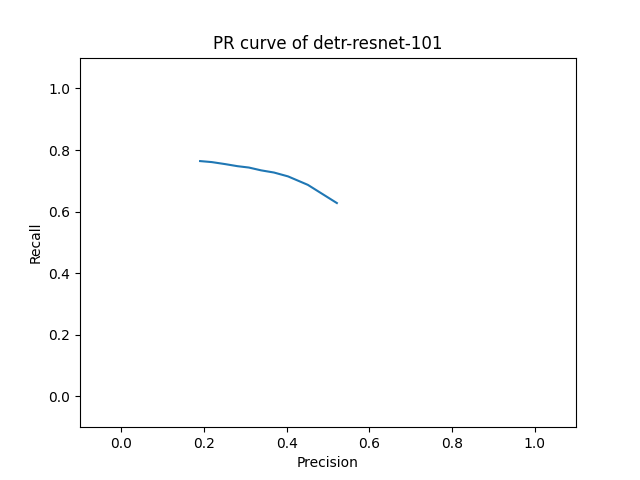
\includegraphics[width=0.49\textwidth]{figures/detr-resnet-101.png}
    \caption{The PR curves of the two DETR models.}
    \label{fig:pr_detr}
\end{figure}


% YN
\begin{table}[h]
    \centering
    \begin{tabular}{|c||c|c|c|c|c|c|c|c|}
        \hline
        CT & MOTA & MOTA\_m & MOTA\_M & MOTP & MT & ML & UO & IDS \\
        \hline
        \hline
        0.9 & 0.01 & 0.00 & 0.22 & nan & 1 & 5886 & 5936 & 43 \\
        \hline
        0.8 & 0.13 & -0.00 & 0.39 & 0.13 & 72 & 4411 & 5936 & 1017 \\
        \hline 
        0.7 & 0.25 & -0.46 & 0.57 & 0.14 & 520 & 2398 & 5936 & 1976 \\
        \hline 
        0.6 & 0.21 & -1.30 & 0.66 & 0.15 & 1143 & 1587 & 5936 & 1709 \\
        \hline 
        0.5 & 0.03 & -4.43 & 0.66 & 0.16 & 1702 & 1208 & 5936 & 1461 \\
        \hline 
        0.4 & -0.26 & -9.61 & 0.68 & 0.16 & 2227 & 1010 & 5936 & 1951 \\
        \hline 
        0.3 & -0.63 & -14.93 & 0.63 & 0.16 & 2583 & 903 & 5936 & 2969 \\
        \hline 
        0.2 & -0.86 & -17.49 & 0.58 & 0.16 & 2717 & 851 & 5936 & 3457 \\
        \hline 
        0.1 & -0.86 & -17.49 & 0.58 & 0.16 & 2717 & 851 & 5936 & 3457 \\
        \hline 
        0.0 & -0.86 & -17.49 & 0.58 & 0.16 & 2717 & 851 & 5936 & 3457 \\
        \hline
    \end{tabular}
    \caption{The performance metrics of the \textbf{YOLOv5 nano}, aggregated across all sequences. CT is the confidence threshold, MOTA is the average MOTA across all sequences, MOTA\_m is the minimum, while MOTA\_M is the maximum achieved on a sequence, MT is the number of mostly tracked trajectories, ML is the number of mostly lost trajectories (it is worth inspecting these in relation with UO - the number of unique object trajectories across all sequences), and IDS is the number of identity switches.}
    \label{tab:mota_yn}
\end{table}
% YS
\begin{table}[h]
    \centering
    \begin{tabular}{|c||c|c|c|c|c|c|c|c|}
        \hline
        CT & MOTA & MOTA\_m & MOTA\_M & MOTP & MT & ML & UO & IDS \\
        \hline
        \hline
        0.9 & 0.03 & 0.00 & 0.28 & nan & 5 & 5705 & 5936 & 248 \\
        \hline
        0.8 & 0.26 & -0.29 & 0.58 & 0.13 & 425 & 2758 & 5936 & 2159 \\
        \hline 
        0.7 & 0.26 & -1.45 & 0.69 & 0.14 & 1343 & 1468 & 5936 & 2087 \\
        \hline 
        0.6 & 0.12 & -2.26 & 0.73 & 0.15 & 2096 & 910 & 5936 & 1673 \\
        \hline 
        0.5 & -0.17 & -6.60 & 0.69 & 0.15 & 2743 & 645 & 5936 & 1819 \\
        \hline 
        0.4 & -0.55 & -12.92 & 0.69 & 0.15 & 3276 & 547 & 5936 & 2981 \\
        \hline 
        0.3 & -1.00 & -19.46 & 0.63 & 0.15 & 3575 & 487 & 5936 & 3934 \\
        \hline 
        0.2 & -1.26 & -22.12 & 0.57 & 0.15 & 3657 & 472 & 5936 & 4181 \\
        \hline 
        0.1 & -1.26 & -22.12 & 0.57 & 0.15 & 3657 & 472 & 5936 & 4181 \\
        \hline 
        0.0 & -1.26 & -22.12 & 0.57 & 0.15 & 3657 & 472 & 5936 & 4181 \\
        \hline 
    \end{tabular}
    \caption{The performance metrics of the \textbf{YOLOv5 small}, aggregated across all sequences. CT is the confidence threshold, MOTA is the average MOTA across all sequences, MOTA\_m is the minimum, while MOTA\_M is the maximum achieved on a sequence, MT is the number of mostly tracked trajectories, ML is the number of mostly lost trajectories (it is worth inspecting these in relation with UO - the number of unique object trajectories across all sequences), and IDS is the number of identity switches.}
    \label{tab:mota_ys}
\end{table}
% YM
\begin{table}[h]
    \centering
    \begin{tabular}{|c||c|c|c|c|c|c|c|c|}
        \hline
        CT & MOTA & MOTA\_m & MOTA\_M & MOTP & MT & ML & UO & IDS \\
        \hline
        \hline
        0.9 & 0.06 & 0.00 & 0.31 & nan & 9 & 5410 & 5936 & 354 \\
        \hline
        0.8 & 0.35 & -0.31 & 0.72 & 0.13 & 1019 & 1573 & 5936 & 1303 \\
        \hline 
        0.7 & 0.23 & -1.89 & 0.80 & 0.14 & 1874 & 917 & 5936 & 1192 \\
        \hline 
        0.6 & -0.05 & -6.69 & 0.70 & 0.14 & 2512 & 618 & 5936 & 1123 \\
        \hline 
        0.5 & -0.37 & -11.63 & 0.73 & 0.15 & 3095 & 505 & 5936 & 1332 \\
        \hline 
        0.4 & -0.70 & -15.28 & 0.71 & 0.15 & 3520 & 445 & 5936 & 1855 \\
        \hline 
        0.3 & -1.06 & -18.25 & 0.68 & 0.15 & 3803 & 407 & 5936 & 2138 \\
        \hline 
        0.2 & -1.29 & -20.29 & 0.64 & 0.15 & 3903 & 402 & 5936 & 2250 \\
        \hline 
        0.1 & -1.29 & -20.29 & 0.64 & 0.15 & 3903 & 402 & 5936 & 2250 \\
        \hline 
        0.0 & -1.29 & -20.29 & 0.64 & 0.15 & 3903 & 402 & 5936 & 2250 \\
        \hline
    \end{tabular}
    \caption{The performance metrics of the \textbf{YOLOv5 medium}, aggregated across all sequences. CT is the confidence threshold, MOTA is the average MOTA across all sequences, MOTA\_m is the minimum, while MOTA\_M is the maximum achieved on a sequence, MT is the number of mostly tracked trajectories, ML is the number of mostly lost trajectories (it is worth inspecting these in relation with UO - the number of unique object trajectories across all sequences), and IDS is the number of identity switches.}
    \label{tab:mota_ym}
\end{table}
% YL
\begin{table}[h]
    \centering
    \begin{tabular}{|c||c|c|c|c|c|c|c|c|}
        \hline
        CT & MOTA & MOTA\_m & MOTA\_M & MOTP & MT & ML & UO & IDS \\
        \hline
        \hline
        0.9 & 0.09 & 0.00 & 0.37 & 0.11 & 27 & 4986 & 5936 & 464 \\
        \hline
        0.8 & 0.33 & -0.97 & 0.80 & 0.14 & 1363 & 1459 & 5936 & 1542 \\
        \hline
        0.7 & 0.14 & -2.68 & 0.81 & 0.14 & 2317 & 850 & 5936 & 1269 \\
        \hline
        0.6 & -0.15 & -6.70 & 0.67 & 0.15 & 2880 & 587 & 5936 & 1171 \\
        \hline
        0.5 & -0.50 & -12.43 & 0.70 & 0.15 & 3341 & 460 & 5936 & 1214 \\
        \hline
        0.4 & -0.83 & -16.11 & 0.69 & 0.15 & 3692 & 403 & 5936 & 1863 \\
        \hline
        0.3 & -1.19 & -18.49 & 0.63 & 0.15 & 3899 & 372 & 5936 & 2120 \\
        \hline
        0.2 & -1.41 & -19.76 & 0.60 & 0.15 & 3956 & 371 & 5936 & 2197 \\
        \hline
        0.1 & -1.41 & -19.76 & 0.60 & 0.15 & 3956 & 371 & 5936 & 2197 \\
        \hline
        0.0 & -1.41 & -19.76 & 0.60 & 0.15 & 3956 & 371 & 5936 & 2197 \\
        \hline
    \end{tabular}
    \caption{The performance metrics of the \textbf{YOLOv5 large}, aggregated across all sequences. CT is the confidence threshold, MOTA is the average MOTA across all sequences, MOTA\_m is the minimum, while MOTA\_M is the maximum achieved on a sequence, MT is the number of mostly tracked trajectories, ML is the number of mostly lost trajectories (it is worth inspecting these in relation with UO - the number of unique object trajectories across all sequences), and IDS is the number of identity switches.}
    \label{tab:mota_yl}
\end{table}
% YX
\begin{table}[h]
    \centering
    \begin{tabular}{|c||c|c|c|c|c|c|c|c|}
        \hline
        CT & MOTA & MOTA\_m & MOTA\_M & MOTP & MT & ML & UO & IDS \\
        \hline
        \hline
        0.9 & 0.14 & -0.17 & 0.47 & 0.11 & 72 & 4455 & 5936 & 633 \\
        \hline
        0.8 & 0.26 & -2.46 & 0.78 & 0.13 & 1323 & 1529 & 5936 & 1204 \\
        \hline
        0.7 & 0.06 & -3.48 & 0.75 & 0.14 & 2079 & 908 & 5936 & 1254 \\
        \hline
        0.6 & -0.26 & -8.14 & 0.65 & 0.14 & 2663 & 596 & 5936 & 1152 \\
        \hline
        0.5 & -0.58 & -13.07 & 0.67 & 0.15 & 3213 & 457 & 5936 & 1483 \\
        \hline
        0.4 & -0.89 & -15.68 & 0.68 & 0.15 & 3635 & 394 & 5936 & 2216 \\
        \hline
        0.3 & -1.24 & -18.04 & 0.65 & 0.15 & 3894 & 370 & 5936 & 2597 \\
        \hline
        0.2 & -1.46 & -19.67 & 0.60 & 0.15 & 3988 & 361 & 5936 & 2695 \\
        \hline
        0.1 & -1.46 & -19.67 & 0.60 & 0.15 & 3988 & 361 & 5936 & 2695 \\
        \hline
        0.0 & -1.46 & -19.67 & 0.60 & 0.15 & 3988 & 361 & 5936 & 2695 \\
        \hline
    \end{tabular}
    \caption{The performance metrics of the \textbf{YOLOv5 extra large}, aggregated across all sequences. CT is the confidence threshold, MOTA is the average MOTA across all sequences, MOTA\_m is the minimum, while MOTA\_M is the maximum achieved on a sequence, MT is the number of mostly tracked trajectories, ML is the number of mostly lost trajectories (it is worth inspecting these in relation with UO - the number of unique object trajectories across all sequences), and IDS is the number of identity switches.}
    \label{tab:mota_yx}
\end{table}
% D50
\begin{table}[h]
    \centering
    \begin{tabular}{|c||c|c|c|c|c|c|c|c|}
        \hline
        CT & MOTA & MOTA\_m & MOTA\_M & MOTP & MT & ML & UO & IDS \\
        \hline
        \hline
        0.9 & -0.42 & -12.51 & 0.74 & 0.16 & 2734 & 814 & 5936 & 1546 \\
        \hline 
        0.8 & -0.75 & -15.65 & 0.73 & 0.16 & 3067 & 723 & 5936 & 1855 \\
        \hline 
        0.7 & -1.00 & -17.71 & 0.73 & 0.16 & 3189 & 680 & 5936 & 2179 \\
        \hline 
        0.6 & -1.20 & -19.20 & 0.71 & 0.16 & 3265 & 654 & 5936 & 2545 \\
        \hline 
        0.5 & -1.38 & -20.38 & 0.70 & 0.16 & 3333 & 630 & 5936 & 2834 \\
        \hline 
        0.4 & -1.55 & -21.49 & 0.69 & 0.17 & 3370 & 622 & 5936 & 3156 \\
        \hline 
        0.3 & -1.75 & -23.09 & 0.67 & 0.17 & 3392 & 616 & 5936 & 3751 \\
        \hline 
        0.2 & -2.01 & -25.55 & 0.63 & 0.17 & 3437 & 614 & 5936 & 4513 \\
        \hline 
        0.1 & -2.45 & -30.64 & 0.57 & 0.17 & 3472 & 598 & 5936 & 6425 \\
        \hline 
        0.0 & -4.66 & -46.39 & 0.09 & 0.17 & 3804 & 429 & 5936 & 21639 \\
        \hline 
    \end{tabular}
    \caption{The performance metrics of the \textbf{DETR-ResNet50}, aggregated across all sequences. CT is the confidence threshold, MOTA is the average MOTA across all sequences, MOTA\_m is the minimum, while MOTA\_M is the maximum achieved on a sequence, MT is the number of mostly tracked trajectories, ML is the number of mostly lost trajectories (it is worth inspecting these in relation with UO - the number of unique object trajectories across all sequences), and IDS is the number of identity switches.}
    \label{tab:mota_detr50}
\end{table}
% D101
\begin{table}[h]
    \centering
    \begin{tabular}{|c||c|c|c|c|c|c|c|c|}
        \hline
        CT & MOTA & MOTA\_m & MOTA\_M & MOTP & MT & ML & UO & IDS \\
        \hline
        \hline
        0.9 & -0.39 & -13.76 & 0.69 & 0.16 & 2758 & 877 & 5936 & 1470 \\
        \hline 
        0.8 & -0.65 & -16.36 & 0.64 & 0.16 & 3072 & 768 & 5936 & 1846 \\
        \hline 
        0.7 & -0.83 & -17.72 & 0.63 & 0.16 & 3211 & 734 & 5936 & 2154 \\
        \hline 
        0.6 & -0.98 & -18.82 & 0.61 & 0.16 & 3289 & 708 & 5936 & 2401 \\
        \hline 
        0.5 & -1.12 & -19.81 & 0.59 & 0.16 & 3345 & 675 & 5936 & 2670 \\
        \hline 
        0.4 & -1.27 & -20.76 & 0.56 & 0.16 & 3393 & 654 & 5936 & 2954 \\
        \hline 
        0.3 & -1.43 & -21.92 & 0.53 & 0.16 & 3431 & 647 & 5936 & 3316 \\
        \hline 
        0.2 & -1.64 & -23.56 & 0.49 & 0.16 & 3446 & 635 & 5936 & 3876 \\
        \hline 
        0.1 & -2.02 & -27.47 & 0.42 & 0.17 & 3484 & 628 & 5936 & 5170 \\
        \hline 
        0.0 & -4.01 & -44.39 & 0.13 & 0.17 & 3730 & 492 & 5936 & 18349 \\
        \hline  
    \end{tabular}
    \caption{The performance metrics of the \textbf{DETR-ResNet101}, aggregated across all sequences. CT is the confidence threshold, MOTA is the average MOTA across all sequences, MOTA\_m is the minimum, while MOTA\_M is the maximum achieved on a sequence, MT is the number of mostly tracked trajectories, ML is the number of mostly lost trajectories (it is worth inspecting these in relation with UO - the number of unique object trajectories across all sequences), and IDS is the number of identity switches.}
    \label{tab:mota_detr101}
\end{table}